% Copyright 2021 Joel Feldman, Andrew Rechnitzer and Elyse Yeager, except where noted.
% This work is licensed under a Creative Commons Attribution-NonCommercial-ShareAlike 4.0 International License.
% https://creativecommons.org/licenses/by-nc-sa/4.0/


 \begin{frame}{Table of Contents}
\mapofcontentsA{\ae}
 \end{frame}
 %--------
\section{1.5 Limits at Infinity}
%----------------------------------------------------------------------------------------
\begin{frame}[t]{End Behavior}

We write:
\[\dlimx{\infty}f(x)=L\]
to express that, as $x$ grows larger and larger, $f(x)$ approaches $L$.\\[1em]
\vfill
Similarly, we write:                                                                                                                                                                                                                                                                                                                                                                                        \[\dlimx{-\infty}f(x)=L\]
to express that, as $x$ grows more and more strongly negative, $f(x)$ approaches $L$.

\pause\vfill
If $L$ is a number, we call $y=L$ a \alert{horizontal asymptote} of $f(x)$.
\unote{Definition~\eref{text}{def_1_5_1}}
\end{frame}
 %--------
%----------------------------------------------------------------------------------------
\begin{frame}{Horizontal Asymptotes}
\begin{center}

\begin{tikzpicture}
\myaxis{x}{5}{5}{y}{1.25}{1.25}
\onslide<1>{\draw (0,0)node{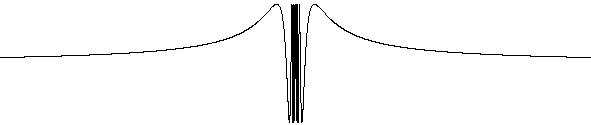
\includegraphics{fig/sin1xHA}};}
\onslide<2|handout:0>{\draw (0,0.4)node{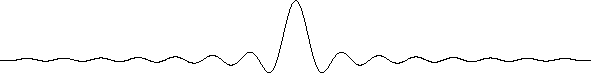
\includegraphics{fig/sinxxHA}};}
\onslide<3|handout:0>{\draw plot[domain=-1.37:1.37,smooth]({tan (\x r)},\x);}
\onslide<4|handout:0>{\draw plot[domain=-5:1,smooth](\x,{exp(\x)-1});}
\end{tikzpicture}
\end{center}\vfill

\only<1>{$y=0$ is a horizontal asymptote for $y=\sin\left(\frac1x\right)$}
\only<2|handout:0>{$y=0$ is a horizontal asymptote for $y=\frac{\sin x}{x}$}
\only<3|handout:0>{$y=\frac{\pi}{2}$ and $y=-\frac{\pi}{2}$ are horizontal asymptotes for $y=\arctan(x)$}
\only<4|handout:0>{$y=-1$ is a horizontal asymptote for $y=e^x-1$}

\note<2>{Don't have to spend a long time on these -- can click through pretty quickly.

Students often think that a HA only occurs when a function gets infinitely close to a value without actually reaching that value}
\note<3>{HA doesn't have to be 0, doesn't have to be the same on both sides, can also have one side with HA and one without}
\StatusBar{1}{4}
\end{frame}
%----------------------------------------------------------------------------------------
\begin{frame}{Common Limits at Infinity}
\AnswerSpace
\only<1>{\AnswerYes \QuestionBar{1}{2}}
\only<2>{\AnswerBar{1}{2}}
\begin{align*}
\dlimx{\infty} 13 &= \onslide<beamer:2-|handout:0>{\alert{13}}
	& \dlimx{\infty}x^3&= \onslide<beamer:2-|handout:0>{\alert{\infty}}\\
\dlimx{-\infty} 13 &= \onslide<beamer:2-|handout:0>{ \alert{13}}
	&\dlimx{-\infty}x^3&=\onslide<beamer:2-|handout:0>{ \alert{-\infty}}\\[2em]
\dlimx{\infty} \frac{1}{x} &=  \onslide<beamer:2-|handout:0>{\alert{0}}
	&\dlimx{-\infty}x^{5/3}&=\onslide<beamer:2-|handout:0>{ \alert{-\infty}}\\
\dlimx{-\infty} \frac{1}{x} &=  \onslide<beamer:2-|handout:0>{\alert{0}}
	&\dlimx{-\infty}x^{2/3}&=\onslide<beamer:2-|handout:0>{ \alert{\infty}}\\[2em]
\dlimx{\infty}x^2&= \onslide<beamer:2-|handout:0>{\alert{\infty}}\\
\dlimx{-\infty}x^2&= \onslide<beamer:2-|handout:0>{\alert{\infty}}
\end{align*}
\end{frame}
%----------------------------------------------------------------------------------------%----------------------------------------------------------------------------------------
\begin{frame}[t]{Arithmetic with Limits at Infinity}
\begin{align*}
\dlimx{\infty}&\left(x+\frac{x^2}{10}  \right)=  \onslide<beamer:2-|handout:0>{\alert{\infty}}\hspace{3cm} \NowYou\\[1em]
\dlimx{\infty}&\left(x-\frac{x^2}{10}  \right)= 
\onslide<beamer:2-|handout:0>{\color{answercolor} \dlimx{\infty}x\left(1-\frac{x}{10}  \right)=  \alert{-\infty}}\\[1em]
\dlimx{-\infty}&\left(x^2+x^3+x^4  \right)=  \onslide<beamer:2-|handout:0>{\color{answercolor}\dlimx{-\infty}x^4\left(\frac{1}{x^2}+\frac{1}{x}+1\right)=\alert{\infty}}\\[1em]
\dlimx{-\infty}&\left(x+13\right)\left(x^2+13\right)^{1/3}=  \onslide<beamer:2-|handout:0>{\alert{-\infty}}
\end{align*}
\only<1>{\AnswerYes \QuestionBar{2}{2}}
\only<2>{\AnswerBar{2}{2}}
\note<1>{Students often have a hard time treating infinity not exactly like a number. Good to point out infinity - infinity isn't necessarily 0, etc. This is a good one to encourage students to chat with their neighbours about. Could also raise hands: who thinks it's 0/inf/-inf, etc.}
\end{frame}
 %--------
%----------------------------------------------------------------------------------------
%----------------------------------------------------------------------------------------
\begin{frame}[t]{Calculating Limits at Infinity}
\[\dlimx{\infty}\frac{x^2+2x+1}{x^3}\]
\only<1-2>{\AnswerYes \QuestionBar{1}{5}} \only<3>{\AnswerBar{1}{5}}
\note<2>{After revealing the trick, can give students some time to start on their own. It should be review.}
\note<3>{Emphasize that we can only do ``arithmetic" like this when the limits individually exist.}
\pause
\only<2|handout:0>{Trick: factor out largest power of denominator.}
\pause\color{answercolor}

\answer{\begin{align*}
\dlimx{\infty}&\frac{x^2+2x+1}{x^3} =
\dlimx{\infty}\frac{x^2+2x+1}{x^3} \left( \frac{\frac{1}{x^3}}{\frac{1}{x^3}}\right)\\
&=\dlimx{\infty}\frac{\frac{1}{x}+\frac{2}{x^2}+\frac{1}{x^3}}{1}
=\frac{\dlimx{\infty}\frac{1}{x}+\dlimx{\infty}\frac{2}{x^2}+\dlimx{\infty}\frac{1}{x^3}}{\dlimx{\infty}1}\\
&=\frac{0+0+0}{1}=\alert{0}
\end{align*}}

\unote{Example~\eref{text}{eg_1_5_2}}
\end{frame}
 %--------
%----------------------------------------------------------------------------------------
%----------------------------------------------------------------------------------------
\begin{frame}[t]{Calculating Limits at Infinity}\AnswerSpace
\only<1-2>{\AnswerYes \QuestionBar{2}{5}} \only<3>{\AnswerBar{2}{5}}
\[\dlimx{-\infty}(x^{7/3}-x^{5/3})\]
\pause
Again: factor out largest power of $x$.\pause\color{answercolor}
\answer{\begin{align*}
(x^{7/3}-x^{5/3})&=
\textcolor{C3}{x^{7/3}}\color{C2}\left(1-\frac{1}{x^{2/3}}\right)\\
\color{C3}\Big(\text{note: }\dlimx{-\infty} x^{7/3}&\color{C3}=-\infty\Big)\\
\color{C2}\Big(\text{note also: }\dlimx{-\infty}\left(1-\frac{1}{x^{2/3}}\right)&\color{C2}=1\Big)
\end{align*}\vfill

So, $\dlimx{-\infty}(x^{7/3}-x^{5/3})=-\infty$}

\unote{Example~\eref{text}{eg_1_5_3}}
\end{frame}
 %--------
%----------------------------------------------------------------------------------------
%----------------------------------------------------------------------------------------
\begin{frame}[t]{Calculating Limits at Infinity}\AnswerSpace
\only<1>{\AnswerYes \QuestionBar{3}{5}} \only<2>{\AnswerBar{3}{5}}
Suppose the height of a bouncing ball is given by $h(t)=\frac{\sin(t)+1}{t}$, for $t \geq 1$. What happens to the height over a long period of time?
\answer{\pause\vfill\color{answercolor}
\begin{align*}
\textcolor{M5}{0} &&\leq&& \textcolor{C3}{\dfrac{\sin(t)+1}{t}} &&\leq&& \textcolor{C4}{\frac{2}{t}}\\
\textcolor{M5}{\lim_{t \rightarrow \infty}0} &&=&& 0 &&=&& \textcolor{C4}{\lim_{t \rightarrow \infty}\frac{2}{t}}
\end{align*}\vfill
So, by the Squeeze Theorem,
\[\color{C3} \lim_{t \rightarrow \infty} \frac{\sin(t)+1}{t}=0\]}
\end{frame}
 %--------
%----------------------------------------------------------------------------------------
%----------------------------------------------------------------------------------------
%----------------------------------------------------------------------------------------
\begin{frame}[t]{Calculating Limits at Infinity}\AnswerSpace
\only<1>{\AnswerYes \QuestionBar{4}{5}} \only<2-4>{\AnswerBar{4}{5}}
\note<1>{It's nice to go over this a few times. Students try; then it goes on the projector; then click through the answer as a review. At each step, talk about how you recognize a situation from before, which helps you decide what to do.}
\only<1-3>{\[\NowYou\hspace{1cm}\dlimx{\infty} \sqrt{x^4+x^2+1}-\sqrt{x^4+3x^2}\]}
\answer{\pause\footnotesize
\color{answercolor}Multiply function by conjugate:\vfill

$\left(\sqrt{x^4+x^2+1}-\sqrt{x^4+3x^2}\right) \left( 
\dfrac{\sqrt{x^4+x^2+1}+\sqrt{x^4+3x^2} }{\sqrt{x^4+x^2+1}+\sqrt{x^4+3x^2} }
\right) $\\
$=\dfrac{-2x^2+1}{\sqrt{x^4+x^2+1}+\sqrt{x^4+3x^2}}$
\pause\vfill

Factor out highest power: $x^2$ (same as $\sqrt{x^4}$)\vfill

$\dfrac{-2x^2+1}{\sqrt{x^4+x^2+1}+\sqrt{x^4+3x^2}}\left(\dfrac{1/x^2}{1/\sqrt{x^4}}\right)$\\
$=\dfrac{-2+\frac{1}{x^2}}{\sqrt{1+\frac{1}{x^2}+\frac{1}{x^4}}+\sqrt{1+\frac{3}{x^2}}}$\pause\vfill

\alert{
$\dlimx{\infty}\dfrac{-2+\frac{1}{x^2}}{\sqrt{1+\frac{1}{x^2}+\frac{1}{x^4}}+\sqrt{1+\frac{3}{x^2}}}=\dfrac{-2+0}{\sqrt{1+0+0}+\sqrt{1+0}}=\frac{-2}{2}=-1$}}
\end{frame}
 %--------



%------------------------------------------------------
\begin{frame}[t]
\only<1>{\AnswerYes \QuestionBar{5}{5}} \only<2>{\AnswerBar{5}{5}}
\note<1>{This is a good one to do in groups (``with your neighbour"). The negative is quite tricky. It helps understanding if students have already tried it on their own. It also brings together several techniques that are probably rusty if not actually brand new.}
\NowYou \qquad Evaluate $\ds\lim_{x \to -\infty}\dfrac{\sqrt{3+x^2}}{3x}$\\[1em]
\pause\color{answercolor}\footnotesize\vfill

\answer{We factor out the largest power of the denominator, which is is $x$.
\begin{align*}
\lim_{x \to -\infty}\dfrac{\sqrt{3+x^2}}{3x}\left(\frac{1/x}{1/x}\right)&=
\lim_{x \to -\infty}\dfrac{\frac{\sqrt{3+x^2}}{x}}{3}
\intertext{When $x<0$, $\sqrt{x^2}=|x|=-x$}
&=
\lim_{x \to -\infty}\dfrac{1}{3}\frac{\sqrt{3+x^2}}{-\sqrt{x^2}}
\\&=
\lim_{x \to -\infty}-\dfrac{1}{3}\sqrt{\frac{3+x^2}{x^2}}
\\&=
\lim_{x \to -\infty}-\dfrac{1}{3}\sqrt{\frac{3}{x^2}+1}\\
&=-\frac{1}{3}
\end{align*}
}
\end{frame}
 %--------
